{\bfseries El tema 3 es una introducción a la minería de datos, especialmente técnicas como el web scrapping y además el aprendizaje 
automatico ligado a estas tecnicas.}

\section{\bfseries Introducción a la minería de datos y aprendizaje automático}

\subsection{\bfseries Minería de datos}
El proceso de minería de datos es un proceso iterativo que consiste en descubrir patrones en grandes volúmenes de datos, inicialmente
se encuentran procesos para preparar y limpiar los datos. El proceso de descubrimiento tiene las siguientes fases:
\begin{itemize}
    \item \textbf{Selección:} Se seleccionan los datos que se van a utilizar.
    \item \textbf{Procesamiento:} Se procesan y limpian para que puedan ser usados de una manera eficiente.
\end{itemize}

\subsection{\bfseries Extracción, transformación y carga de datos (ETL)}
Básicamente, el proceso ETL se encarga de extraer datos de diferentes fuentes, transformarlos y cargarlos en un almacén de datos.
Esta será una palabra que se escuchará mucho en el mundo de la minería de datos, ya que es un proceso fundamental para este.

\begin{tcolorbox}[title=Proceso de ETL]
\centering
\begin{tikzpicture}[node distance=0.5cm and 0.5cm, scale=0.8, every node/.style={scale=0.8}]

% Nodes for ETL process
\node[data] (data) {Datos};
\node[process, below right=0.3cm and 0.3cm of data] (selection) {Selecci\'on};
\node[data, below right=0.3cm and 0.3cm of selection] (selected) {Datos seleccionados};
\node[process, below right=0.3cm and 0.3cm of selected] (processing) {Procesamiento};
\node[data, below right=0.3cm and 0.3cm of processing] (processed) {Datos procesados};
\node[process, below right=0.3cm and 0.3cm of processed] (transformation) {Transformaci\'on};
\node[output, below right=0.3cm and 0.3cm of transformation] (transformed) {Datos transformados};


% Arrows for ETL
\draw[arrow] (data) -- (selection);
\draw[arrow] (selection) -- (selected);
\draw[arrow] (selected) -- (processing);
\draw[arrow] (processing) -- (processed);
\draw[arrow] (processed) -- (transformation);
\draw[arrow] (transformation) -- (transformed);


\end{tikzpicture}

\end{tcolorbox}

\subsection{\bfseries Aprendizaje automático}

El aprendizaje automático es una rama de la inteligencia artificial que permite a las máquinas aprender de los datos y hacer predicciones o tomar decisiones sin ser programadas explícitamente para ello. Existen varios tipos de aprendizaje automático:

\begin{itemize}
    \item \textbf{Aprendizaje supervisado:} Se entrena un modelo con datos etiquetados, es decir, datos que ya tienen una respuesta conocida.
    \item \textbf{Aprendizaje no supervisado:} Se entrena un modelo con datos no etiquetados y el objetivo es encontrar patrones o estructuras ocultas en los datos.
    \item \textbf{Aprendizaje semi-supervisado:} Combina una pequeña cantidad de datos etiquetados con una gran cantidad de datos no etiquetados durante el entrenamiento.
    \item \textbf{Aprendizaje por refuerzo:} Un agente aprende a tomar decisiones mediante la interacción con un entorno y la obtención de recompensas o castigos.
\end{itemize}


\section{\bfseries Extracción, transformación y carga de datos}

Antes de realizar web scrapping; \textbf{¿Es legal?}, sorprendentemente si, pero siguiendo diferentes reglas y normas:
\begin{multicols}{2}
    \begin{itemize}
        \item La información tiene que ser pública.
        \item Tienes que aceptar explícitamente los terminos de uso.
        \item Puedo hacer uso de los datos siempre que no lesione los derechos de autor.
    \end{itemize}
\end{multicols}

\subsection{\bfseries APIs}

Una API es un canal de comunicación, que permite que 2 software se comuniquen entre sí. Tiene 4 tipos diferentes de peticiones:
\begin{tcolorbox}[title=Peticiones API]
    \begin{itemize}
        \item \textbf{GET:} Se utiliza para obtener datos de un servidor.
        \item \textbf{POST:} Se utiliza para enviar datos a un servidor.
        \item \textbf{PUT:} Se utiliza para actualizar datos en un servidor.
        \item \textbf{DELETE:} Se utiliza para eliminar datos de un servidor.
    \end{itemize}
\end{tcolorbox}

Estas peticiones se realizan contra endpoints, que son formas de interactuar con este. También cabe destacar \textbf{REST}, que es un estilo de arquitectura de software que define un conjunto de restricciones para crear servicios web.

\textbf{\large Ejemplo:} 
\begin{lstlisting}[language=Python]
    import requests
    url = 'https://pokeapi.co/api/v2/pokemon/ditto'

    response = requests.get(url)
    print(response.json())
\end{lstlisting}

  En el ejemplo de encima hacemos un request a la API de Pokemon, y obtenemos la información del Pokemon Ditto. Dependiendo de la respuesta que nos encontremos, esta nos informa de si la petición ha sido correcta o no. Estas respuestas se dividen en diferentes códigos de estado:
  \begin{multicols}{2}
    \begin{itemize}
        \item 1xx: Información
        \item 2xx: Éxito
        \item 3xx: Redirección
        \item 4xx: Error del cliente
        \item 5xx: Error del servidor
    \end{itemize}
  \end{multicols}

Pero aqui nos encontramos un problema, ya que no es común que las APIs tengan una documentación clara y concisa, o directamente ni siquiera
ni nos permitan hacer uso de ellas. Para acceder a una API que no tiene una documentación clara, podemos hacer uso de la técnica de web scrapping o parsear el HTML directamente con BS4. \newline
\textbf{\large Ejemplo con BS4:} 
\begin{lstlisting}[language=Python]
    #Ejemplo con BeautifulSoup y la wikipedia de la UEM
    from bs4 import BeautifulSoup

    url = 'https://es.wikipedia.org/wiki/Universidad_Europea_de_Madrid'
    response = requests.get(url)
    soup = BeautifulSoup(response.content,"html.parser")
\end{lstlisting}

\section{\bfseries Representación y visualización de datos}
La representación de datos es una parte fundamental en la minería de datos, ya que nos permite visualizar los datos y darles un enfoque
diferente. Ya que aunque un analisis pueda tener datos muy similares, una vez visualizados estos pueden tener un enfoque diferente. Esto, por ejemplo
, se hace muy fácil de ver en el \textbf{Cuarteto de Anscombe}:

\begin{figure}[htbp]
    \centering
    \begin{minipage}{0.4\textwidth}
        \centering
        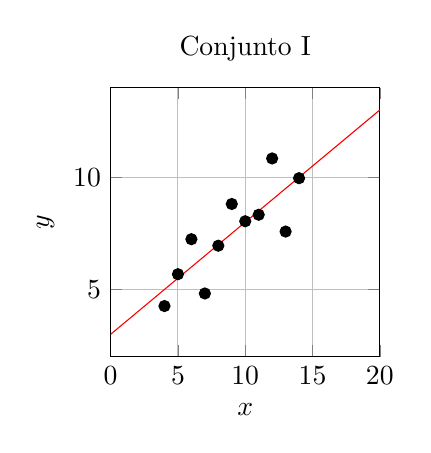
\begin{tikzpicture}
        \begin{axis}[
            title={Conjunto I},
            width=5cm, height=5cm, % Dimensiones más pequeñas
            xlabel={$x$}, ylabel={$y$},
            grid=major,
            xmin=0, xmax=20, ymin=2, ymax=14
        ]
        \addplot[only marks] coordinates {
            (10, 8.04) (8, 6.95) (13, 7.58) (9, 8.81) 
            (11, 8.33) (14, 9.96) (6, 7.24) (4, 4.26) 
            (12, 10.84) (7, 4.82) (5, 5.68)
        };
        \addplot[domain=0:20, red] {0.5 * x + 3};
        \end{axis}
        \end{tikzpicture}
    \end{minipage}
    \hfill
    \begin{minipage}{0.4\textwidth}
        \centering
        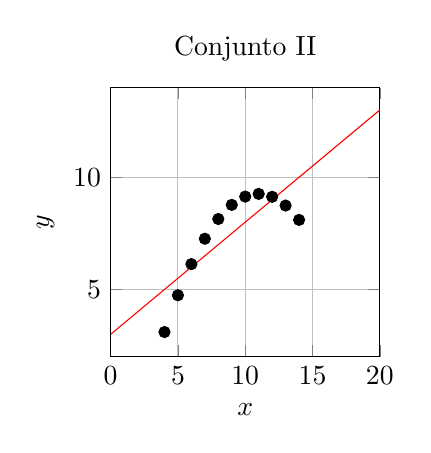
\begin{tikzpicture}
        \begin{axis}[
            title={Conjunto II},
            width=5cm, height=5cm, % Dimensiones más pequeñas
            xlabel={$x$}, ylabel={$y$},
            grid=major,
            xmin=0, xmax=20, ymin=2, ymax=14
        ]
        \addplot[only marks] coordinates {
            (10, 9.14) (8, 8.14) (13, 8.74) (9, 8.77) 
            (11, 9.26) (14, 8.10) (6, 6.13) (4, 3.10) 
            (12, 9.13) (7, 7.26) (5, 4.74)
        };
        \addplot[domain=0:20, red] {0.5 * x + 3};
        \end{axis}
        \end{tikzpicture}
    \end{minipage}

    \vspace{0.5cm}

    \begin{minipage}{0.4\textwidth}
        \centering
        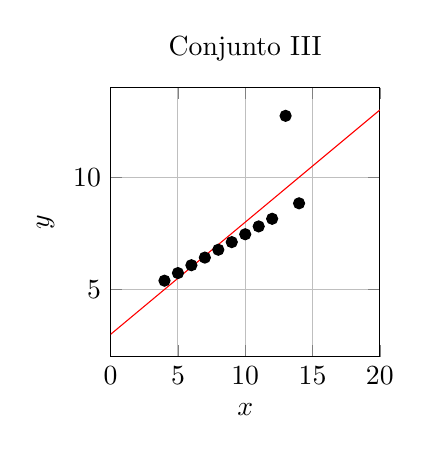
\begin{tikzpicture}
        \begin{axis}[
            title={Conjunto III},
            width=5cm, height=5cm, % Dimensiones más pequeñas
            xlabel={$x$}, ylabel={$y$},
            grid=major,
            xmin=0, xmax=20, ymin=2, ymax=14
        ]
        \addplot[only marks] coordinates {
            (10, 7.46) (8, 6.77) (13, 12.74) (9, 7.11) 
            (11, 7.81) (14, 8.84) (6, 6.08) (4, 5.39) 
            (12, 8.15) (7, 6.42) (5, 5.73)
        };
        \addplot[domain=0:20, red] {0.5 * x + 3};
        \end{axis}
        \end{tikzpicture}
    \end{minipage}
    \hfill
    \begin{minipage}{0.4\textwidth}
        \centering
        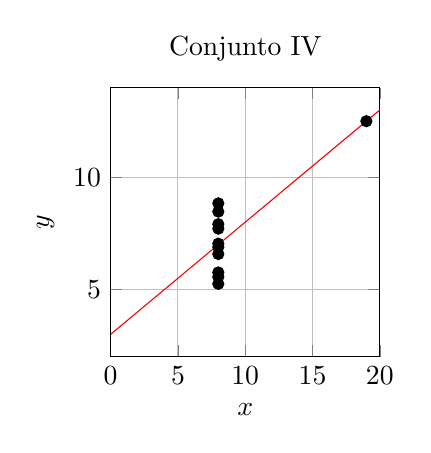
\begin{tikzpicture}
        \begin{axis}[
            title={Conjunto IV},
            width=5cm, height=5cm, % Dimensiones más pequeñas
            xlabel={$x$}, ylabel={$y$},
            grid=major,
            xmin=0, xmax=20, ymin=2, ymax=14
        ]
        \addplot[only marks] coordinates {
            (8, 6.58) (8, 5.76) (8, 7.71) (8, 8.84) 
            (8, 8.47) (8, 7.04) (8, 5.25) (19, 12.50) 
            (8, 5.56) (8, 7.91) (8, 6.89)
        };
        \addplot[domain=0:20, red] {0.5 * x + 3};
        \end{axis}
        \end{tikzpicture}
    \end{minipage}
\end{figure}

Todos estos gráficos tienen datos muy similares (media, varianza, correlación\ldots) pero sus representaciones gráficas son totalmente diferentes.
Esto nos demuestra la importancia de la representación de datos para poder comprender una función o un conjunto de datos.